\chapter{Introduction}

This manual has been written to give an overview over the functionality of the \ogs Data Explorer. Existing functionality is explained and typical workflows are detailed step by step.

\bigskip

\ogs (formerly Rockflow) is a programme for the simulation of (coupled) thermal, hydrological, mechanical and chemical processes. Over various iterations the software is about $20$ years old and compiles a large amount of functionality, interfaces and numerical solvers. It is, however, a command line tool. Therefore, it is difficult to get a feeling for the data that is handled by the programme and simulation results cannot be directly verified without the help of other tools.

The \ogs Data Explorer is a graphical user interface (GUI) has been developed to fill that gap and provides a means for the visualisation of data. It employs the same basic data structures as the command line tool and thus complements \ogs by giving the user a way to visually assess the data and see possible errors, inconsistencies or missing information.

However, it is important to keep in mind that the \ogs Data Explorer is \emph{not} a fully developed tool with a defined scope of functionality. Features are constantly being added and while everyone is making an effort to keep things as straightforward and robust as possible, it can be difficult to find out what the programme is currently capable of and how exactly things need to be done.

This manual will give you an overview of the features of the programme, how things work and what possible problems you might encounter. For more information on \ogs itself check out the OGS-Wiki\footnote{https://svn.ufz.de/ogs}.\index{OGS Wiki}

It is also highly recommended to always use the latest version which is always available on the Jenkins \index{Jenkins Build Server} Buildserver\footnote{https://svn.ufz.de/hudson}\footnote{http://jenkins-ci.org/}.

\subsection*{Important concepts}

\begin{figure}[tb]
\begin{center}
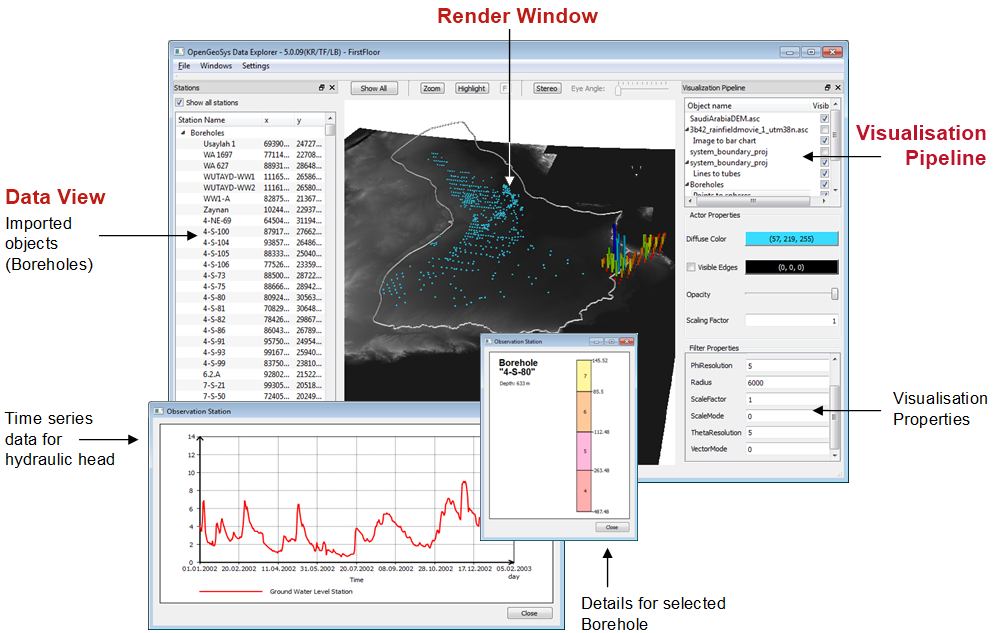
\includegraphics[width=0.99\linewidth]{gui}
\caption{The graphical user interface of the \ogs Data Explorer.}
\label{fig:gui}
\end{center}
\end{figure}

In the following a number of terms will appear over and over again and it is important to know what they mean, to be able to follow the instructions.

Figure \ref{fig:gui} shows a screenshot of the GUI of the \ogs Data Explorer. The three most important parts of the user interface are marked as ``Data View'', ``Render Window'' and ``Visualisation Pipeline''. These elements and the information they contained are explained in detail in section \ref{datavisualisation} and the names will pop up again and again in this manual so it is important that you know what is meant if you read the names.

\ogs is a tool that is written in a programming language called C++. As many other programming language it allows the developer to add so called libraries that define a certain set of functionality. This means a programmer does not need to implement every function provided by a programme himself but this function is instead provided by the library and can be used by anyone linking to that library. The Data Explorer makes use of a number of such libraries. The two most important ones are called Qt\footnote{http://qt.nokia.com} and VTK\footnote{http://www.vtk.org}.

Qt\index{Qt} is a library mainly providing functionality for a user interface, i.e. the definition of windows, dialogs and everything you expect to see in there, such as buttons, lists, menus, etc. Qt offers a lot more than that but explaining it all would go beyond the scope of this manual. Elements of the Data Explorer that make use of Qt are for instance the ``Data View'' or the windows displaying diagrams or borehole stratigraphies.

VTK\index{VTK} (Visualisation Toolkit) is a graphics library which can be used for the visualisation of objects in 3D. It can also save these 3D objects in files, which in turn are called VTK-files and can also be used by the Data Explorer. The ``Render Window'' and anything that is displayed there has been constructed using VTK.

